\begin{figure}[H]
\centering
\begin{tikzpicture}
\begin{groupplot}[
  group style={group size=2 by 2, horizontal sep=1.4cm, vertical sep=1.5cm,
    xlabels at=edge bottom, ylabels at=edge left},
  width=0.46\textwidth, height=4.2cm,
  ymin=0, ymax=1.05, xmin=5, xmax=50,
  xtick={5,20,35,50},
  ylabel={Acurácia ponderada},
  xlabel={$N$ (nós)},
  grid=major, grid style={dotted,gray!40},
  legend style={font=\tiny, draw=none, fill=none, legend columns=4,
    at={(0.5,1.18)}, anchor=south, /tikz/every even column/.append style={column sep=4pt}},
  mark size=1.1pt, line width=0.7pt]
\nextgroupplot[title={\small Sem conluio}]
  \addplot+[mark=*] coordinates {(5,0.9993) (10,1.0000) (15,1.0000) (20,1.0000) (25,1.0000) (30,1.0000) (35,1.0000) (40,1.0000) (45,1.0000) (50,1.0000)};
  \addlegendentry{0\%}
  \addplot+[mark=*] coordinates {(5,0.9960) (10,1.0000) (15,1.0000) (20,1.0000) (25,1.0000) (30,1.0000) (35,1.0000) (40,1.0000) (45,1.0000) (50,1.0000)};
  \addlegendentry{5\%}
  \addplot+[mark=*] coordinates {(5,0.9960) (10,1.0000) (15,1.0000) (20,1.0000) (25,1.0000) (30,1.0000) (35,1.0000) (40,1.0000) (45,1.0000) (50,1.0000)};
  \addlegendentry{20\%}
  \addplot+[mark=*] coordinates {(5,0.9960) (10,1.0000) (15,1.0000) (20,1.0000) (25,1.0000) (30,1.0000) (35,1.0000) (40,1.0000) (45,1.0000) (50,1.0000)};
  \addlegendentry{35\%}
  \addplot+[mark=*] coordinates {(5,0.9773) (10,0.9907) (15,1.0000) (20,1.0000) (25,1.0000) (30,1.0000) (35,1.0000) (40,1.0000) (45,1.0000) (50,1.0000)};
  \addlegendentry{50\%}
  \addplot+[mark=*] coordinates {(5,0.7427) (10,0.9560) (15,0.9880) (20,0.9827) (25,0.9947) (30,0.9993) (35,1.0000) (40,0.9993) (45,1.0000) (50,1.0000)};
  \addlegendentry{65\%}
  \addplot+[mark=*] coordinates {(5,0.2367) (10,0.5040) (15,0.5553) (20,0.6120) (25,0.6927) (30,0.7160) (35,0.7833) (40,0.8273) (45,0.8627) (50,0.8820)};
  \addlegendentry{80\%}
\nextgroupplot[title={\small Com conluio}]
  \addplot+[mark=*, forget plot] coordinates {(5,0.9953) (10,1.0000) (15,1.0000) (20,1.0000) (25,1.0000) (30,1.0000) (35,1.0000) (40,1.0000) (45,1.0000) (50,1.0000)};
  \addplot+[mark=*, forget plot] coordinates {(5,0.9953) (10,1.0000) (15,1.0000) (20,1.0000) (25,1.0000) (30,1.0000) (35,1.0000) (40,1.0000) (45,1.0000) (50,1.0000)};
  \addplot+[mark=*, forget plot] coordinates {(5,0.9953) (10,1.0000) (15,1.0000) (20,1.0000) (25,1.0000) (30,1.0000) (35,1.0000) (40,1.0000) (45,1.0000) (50,1.0000)};
  \addplot+[mark=*, forget plot] coordinates {(5,0.9947) (10,1.0000) (15,1.0000) (20,1.0000) (25,1.0000) (30,1.0000) (35,1.0000) (40,1.0000) (45,1.0000) (50,1.0000)};
  \addplot+[mark=*, forget plot] coordinates {(5,0.9747) (10,0.6007) (15,0.7933) (20,0.3467) (25,0.6087) (30,0.2153) (35,0.4493) (40,0.1187) (45,0.2867) (50,0.0793)};
  \addplot+[mark=*, forget plot] coordinates {(5,0.0000) (10,0.0000) (15,0.0000) (20,0.0000) (25,0.0000) (30,0.0000) (35,0.0000) (40,0.0000) (45,0.0000) (50,0.0000)};
  \addplot+[mark=*, forget plot] coordinates {(5,0.0000) (10,0.0000) (15,0.0000) (20,0.0000) (25,0.0000) (30,0.0000) (35,0.0000) (40,0.0000) (45,0.0000) (50,0.0000)};
\nextgroupplot[title={\small Sem + inst.}]
  \addplot+[mark=*, forget plot] coordinates {(5,0.9967) (10,1.0000) (15,1.0000) (20,1.0000) (25,1.0000) (30,1.0000) (35,1.0000) (40,1.0000) (45,1.0000) (50,1.0000)};
  \addplot+[mark=*, forget plot] coordinates {(5,0.9987) (10,1.0000) (15,1.0000) (20,1.0000) (25,1.0000) (30,1.0000) (35,1.0000) (40,1.0000) (45,1.0000) (50,1.0000)};
  \addplot+[mark=*, forget plot] coordinates {(5,0.9927) (10,1.0000) (15,1.0000) (20,1.0000) (25,1.0000) (30,1.0000) (35,1.0000) (40,1.0000) (45,1.0000) (50,1.0000)};
  \addplot+[mark=*, forget plot] coordinates {(5,0.9933) (10,1.0000) (15,1.0000) (20,1.0000) (25,1.0000) (30,1.0000) (35,1.0000) (40,1.0000) (45,1.0000) (50,1.0000)};
  \addplot+[mark=*, forget plot] coordinates {(5,0.9847) (10,0.9987) (15,1.0000) (20,1.0000) (25,1.0000) (30,1.0000) (35,1.0000) (40,1.0000) (45,1.0000) (50,1.0000)};
  \addplot+[mark=*, forget plot] coordinates {(5,0.8700) (10,0.9967) (15,1.0000) (20,0.9993) (25,1.0000) (30,1.0000) (35,1.0000) (40,1.0000) (45,1.0000) (50,1.0000)};
  \addplot+[mark=*, forget plot] coordinates {(5,0.4120) (10,0.7960) (15,0.8980) (20,0.9480) (25,0.9667) (30,0.9793) (35,0.9907) (40,0.9967) (45,0.9980) (50,0.9980)};
\nextgroupplot[title={\small Com + inst.}]
  \addplot+[mark=*, forget plot] coordinates {(5,0.9980) (10,1.0000) (15,1.0000) (20,1.0000) (25,1.0000) (30,1.0000) (35,1.0000) (40,1.0000) (45,1.0000) (50,1.0000)};
  \addplot+[mark=*, forget plot] coordinates {(5,1.0000) (10,1.0000) (15,1.0000) (20,1.0000) (25,1.0000) (30,1.0000) (35,1.0000) (40,1.0000) (45,1.0000) (50,1.0000)};
  \addplot+[mark=*, forget plot] coordinates {(5,0.9907) (10,1.0000) (15,1.0000) (20,1.0000) (25,1.0000) (30,1.0000) (35,1.0000) (40,1.0000) (45,1.0000) (50,1.0000)};
  \addplot+[mark=*, forget plot] coordinates {(5,0.9907) (10,1.0000) (15,1.0000) (20,1.0000) (25,1.0000) (30,1.0000) (35,1.0000) (40,1.0000) (45,1.0000) (50,1.0000)};
  \addplot+[mark=*, forget plot] coordinates {(5,0.9840) (10,0.9987) (15,1.0000) (20,1.0000) (25,1.0000) (30,1.0000) (35,1.0000) (40,1.0000) (45,1.0000) (50,1.0000)};
  \addplot+[mark=*, forget plot] coordinates {(5,0.9033) (10,0.9973) (15,0.9940) (20,0.8633) (25,0.9727) (30,0.9007) (35,0.9880) (40,0.8400) (45,0.8007) (50,0.9227)};
  \addplot+[mark=*, forget plot] coordinates {(5,0.3920) (10,0.1500) (15,0.0247) (20,0.0140) (25,0.0073) (30,0.0107) (35,0.0047) (40,0.0027) (45,0.0040) (50,0.0013)};
\end{groupplot}
\end{tikzpicture}
\caption{Acurácia do consenso ponderado em função de $N$ (média de 30 sementes).}
\label{fig:acuracia-n}
\end{figure}

\begin{figure}[H]
\centering
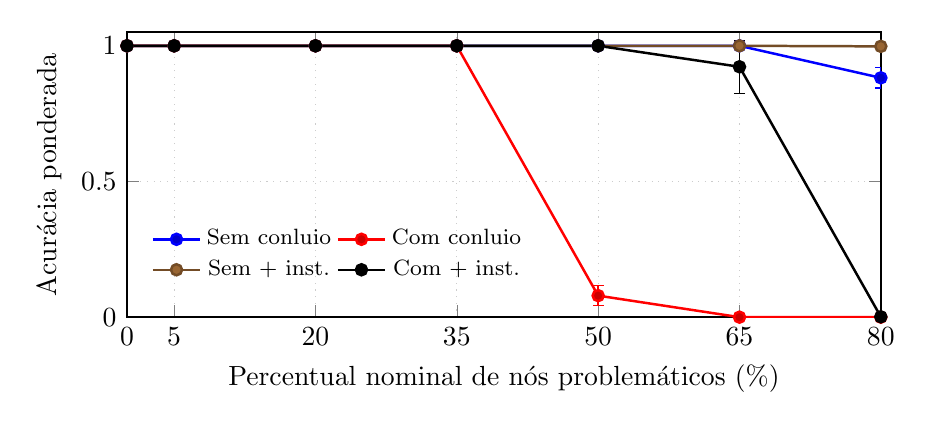
\begin{tikzpicture}
\begin{axis}[
  width=0.92\textwidth, height=5.2cm,
  ymin=0, ymax=1.05, xmin=0, xmax=80,
  xtick={0,5,20,35,50,65,80},
  xlabel={Percentual nominal de nós problemáticos (\%)},
  ylabel={Acurácia ponderada},
  grid=major, grid style={dotted,gray!40},
  legend style={font=\footnotesize, draw=none, fill=none, legend columns=2,
    at={(0.02,0.22)}, anchor=west},
  mark size=2pt, line width=0.9pt, error bars/y dir=both,
  error bars/y explicit, error bars/error bar style={line width=0.5pt}]
  \addplot+[mark=*] coordinates {(0,1.0000) +- (0,0.0000) (5,1.0000) +- (0,0.0000) (20,1.0000) +- (0,0.0000) (35,1.0000) +- (0,0.0000) (50,1.0000) +- (0,0.0000) (65,1.0000) +- (0,0.0000) (80,0.8820) +- (0,0.0373)};
  \addlegendentry{Sem conluio}
  \addplot+[mark=*] coordinates {(0,1.0000) +- (0,0.0000) (5,1.0000) +- (0,0.0000) (20,1.0000) +- (0,0.0000) (35,1.0000) +- (0,0.0000) (50,0.0793) +- (0,0.0369) (65,0.0000) +- (0,0.0000) (80,0.0000) +- (0,0.0000)};
  \addlegendentry{Com conluio}
  \addplot+[mark=*] coordinates {(0,1.0000) +- (0,0.0000) (5,1.0000) +- (0,0.0000) (20,1.0000) +- (0,0.0000) (35,1.0000) +- (0,0.0000) (50,1.0000) +- (0,0.0000) (65,1.0000) +- (0,0.0000) (80,0.9980) +- (0,0.0061)};
  \addlegendentry{Sem + inst.}
  \addplot+[mark=*] coordinates {(0,1.0000) +- (0,0.0000) (5,1.0000) +- (0,0.0000) (20,1.0000) +- (0,0.0000) (35,1.0000) +- (0,0.0000) (50,1.0000) +- (0,0.0000) (65,0.9227) +- (0,0.0971) (80,0.0013) +- (0,0.0051)};
  \addlegendentry{Com + inst.}
\end{axis}
\end{tikzpicture}
\caption{Acurácia ponderada em $N=50$ nos sete percentuais nominais (média $\pm$ desvio, 30 sementes).}
\label{fig:n50-panorama}
\end{figure}

\begin{figure}[H]
\centering
\begin{tikzpicture}
\begin{groupplot}[
  group style={group size=2 by 2, horizontal sep=1.3cm, vertical sep=1.4cm,
    xlabels at=edge bottom, ylabels at=edge left},
  width=0.46\textwidth, height=4.0cm,
  ymin=0, ymax=1.05, xmin=0, xmax=50,
  ylabel={Reputação média}, xlabel={Rodada},
  grid=major, grid style={dotted,gray!40},
  legend style={font=\tiny, draw=none, fill=none, legend columns=3,
    at={(0.5,1.16)}, anchor=south},
  mark size=1.0pt, line width=0.8pt]
\nextgroupplot[title={\small Sem conluio}]
  \addplot[solid, mark=o, color=blue!70!black] coordinates {(0,0.5000) (2,0.5000) (4,0.5000) (6,0.5000) (8,0.5000) (10,0.5000) (12,0.5000) (14,0.5000) (16,0.5000) (18,0.5000) (20,0.5000) (22,0.5000) (24,0.5000) (26,0.5000) (28,0.5000) (30,0.5000) (32,0.5000) (34,0.5000) (36,0.5000) (38,0.5000) (40,0.5000) (42,0.5000) (44,0.5000) (46,0.5000) (48,0.5000) (49,0.5000)};
  \addlegendentry{Honestos}
  \addplot[dashed, mark=square, color=red!70!black] coordinates {(0,0.5000) (2,0.5000) (4,0.5000) (6,0.5000) (8,0.5000) (10,0.5000) (12,0.5000) (14,0.5000) (16,0.5000) (18,0.5000) (20,0.5000) (22,0.5000) (24,0.5000) (26,0.5000) (28,0.5000) (30,0.5000) (32,0.5000) (34,0.5000) (36,0.5000) (38,0.5000) (40,0.5000) (42,0.5000) (44,0.5000) (46,0.5000) (48,0.5000) (49,0.5000)};
  \addlegendentry{Maliciosos}
\nextgroupplot[title={\small Com conluio}]
  \addplot[solid, mark=o, color=blue!70!black, forget plot] coordinates {(0,0.5000) (2,0.5000) (4,0.5000) (6,0.5000) (8,0.5000) (10,0.5000) (12,0.5000) (14,0.5000) (16,0.5000) (18,0.5000) (20,0.5000) (22,0.5000) (24,0.5000) (26,0.5000) (28,0.5000) (30,0.5000) (32,0.5000) (34,0.5000) (36,0.5000) (38,0.5000) (40,0.5000) (42,0.5000) (44,0.5000) (46,0.5000) (48,0.5000) (49,0.5000)};
  \addplot[dashed, mark=square, color=red!70!black, forget plot] coordinates {(0,0.5000) (2,0.5000) (4,0.5000) (6,0.5000) (8,0.5000) (10,0.5000) (12,0.5000) (14,0.5000) (16,0.5000) (18,0.5000) (20,0.5000) (22,0.5000) (24,0.5000) (26,0.5000) (28,0.5000) (30,0.5000) (32,0.5000) (34,0.5000) (36,0.5000) (38,0.5000) (40,0.5000) (42,0.5000) (44,0.5000) (46,0.5000) (48,0.5000) (49,0.5000)};
  \node[font=\tiny, align=center, fill=white, fill opacity=0.85, inner sep=1pt]    at (axis cs:38,0.52) {Empate / hold};
\nextgroupplot[title={\small Sem + inst.}]
  \addplot[solid, mark=o, color=blue!70!black, forget plot] coordinates {(0,0.5778) (2,0.7095) (4,0.7935) (6,0.8409) (8,0.8613) (10,0.8803) (12,0.8909) (14,0.8961) (16,0.8973) (18,0.8938) (20,0.8984) (22,0.8959) (24,0.8938) (26,0.9044) (28,0.9039) (30,0.9019) (32,0.9051) (34,0.9045) (36,0.9032) (38,0.8966) (40,0.8996) (42,0.9002) (44,0.9028) (46,0.8937) (48,0.8899) (49,0.8951)};
  \addplot[dashed, mark=square, color=red!70!black, forget plot] coordinates {(0,0.4042) (2,0.2401) (4,0.1351) (6,0.0759) (8,0.0427) (10,0.0240) (12,0.0135) (14,0.0076) (16,0.0043) (18,0.0024) (20,0.0014) (22,0.0008) (24,0.0004) (26,0.0002) (28,0.0001) (30,0.0001) (32,0.0000) (34,0.0000) (36,0.0000) (38,0.0000) (40,0.0000) (42,0.0000) (44,0.0000) (46,0.0000) (48,0.0000) (49,0.0000)};
  \addplot[dotted, mark=triangle, color=orange!80!black, forget plot] coordinates {(0,0.4639) (2,0.4185) (4,0.3960) (6,0.3714) (8,0.3596) (10,0.3623) (12,0.3573) (14,0.3583) (16,0.3531) (18,0.3444) (20,0.3472) (22,0.3557) (24,0.3549) (26,0.3584) (28,0.3530) (30,0.3489) (32,0.3554) (34,0.3371) (36,0.3400) (38,0.3310) (40,0.3530) (42,0.3566) (44,0.3481) (46,0.3439) (48,0.3426) (49,0.3375)};
\nextgroupplot[title={\small Com + inst.}]
  \addplot[solid, mark=o, color=blue!70!black, forget plot] coordinates {(0,0.5720) (2,0.7077) (4,0.7942) (6,0.8396) (8,0.8696) (10,0.8766) (12,0.8846) (14,0.8944) (16,0.8942) (18,0.8941) (20,0.8992) (22,0.8992) (24,0.9022) (26,0.9056) (28,0.9016) (30,0.9018) (32,0.9012) (34,0.8999) (36,0.8969) (38,0.8961) (40,0.8945) (42,0.8966) (44,0.9000) (46,0.8999) (48,0.9029) (49,0.9045)};
  \addplot[dashed, mark=square, color=red!70!black, forget plot] coordinates {(0,0.4167) (2,0.2445) (4,0.1376) (6,0.0774) (8,0.0435) (10,0.0245) (12,0.0138) (14,0.0078) (16,0.0044) (18,0.0024) (20,0.0014) (22,0.0008) (24,0.0004) (26,0.0002) (28,0.0001) (30,0.0001) (32,0.0000) (34,0.0000) (36,0.0000) (38,0.0000) (40,0.0000) (42,0.0000) (44,0.0000) (46,0.0000) (48,0.0000) (49,0.0000)};
  \addplot[dotted, mark=triangle, color=orange!80!black, forget plot] coordinates {(0,0.4663) (2,0.4128) (4,0.4034) (6,0.3880) (8,0.3783) (10,0.3788) (12,0.3655) (14,0.3697) (16,0.3748) (18,0.3622) (20,0.3438) (22,0.3488) (24,0.3542) (26,0.3589) (28,0.3509) (30,0.3611) (32,0.3587) (34,0.3577) (36,0.3607) (38,0.3461) (40,0.3589) (42,0.3536) (44,0.3566) (46,0.3582) (48,0.3643) (49,0.3739)};
\end{groupplot}
\end{tikzpicture}
\caption{Reputação média por perfil em $N=50$ e 50\% de nós problemáticos.}
\label{fig:n50-p50-rep}
\end{figure}

\begin{figure}[H]
\centering
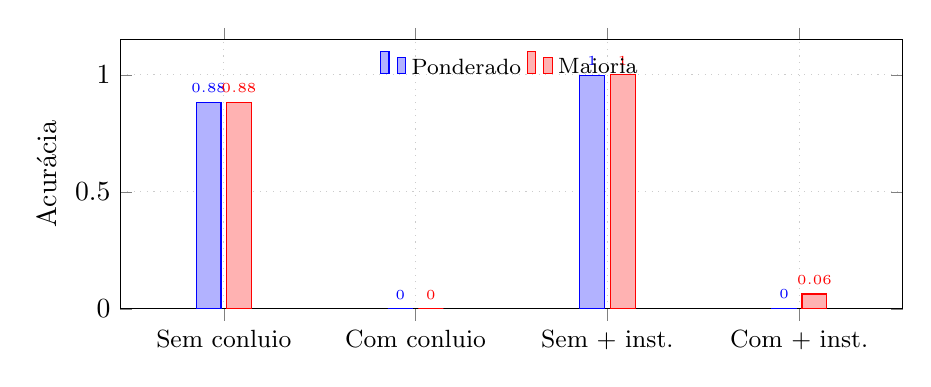
\begin{tikzpicture}
\begin{axis}[
  ybar, bar width=9pt,
  width=0.95\textwidth, height=5.0cm,
  ymin=0, ymax=1.15,
  ylabel={Acurácia},
  symbolic x coords={Sem conluio, Com conluio, Sem + inst., Com + inst.},
  xtick=data, x tick label style={font=\small},
  enlarge x limits=0.18,
  grid=major, grid style={dotted,gray!40},
  legend style={font=\footnotesize, draw=none, fill=none, at={(0.5,0.98)},
    anchor=north, legend columns=2},
  nodes near coords, nodes near coords style={font=\tiny, /pgf/number format/fixed,
    /pgf/number format/precision=2}]
  \addplot coordinates {({Sem conluio},0.8820) ({Com conluio},0.0000) ({Sem + inst.},0.9980) ({Com + inst.},0.0013)};
  \addlegendentry{Ponderado}
  \addplot coordinates {({Sem conluio},0.8820) ({Com conluio},0.0000) ({Sem + inst.},1.0000) ({Com + inst.},0.0640)};
  \addlegendentry{Maioria}
\end{axis}
\end{tikzpicture}
\caption{Acurácia ponderada e por maioria em $N=50$ e 80\% nominal, nas quatro configurações (30 sementes).}
\label{fig:n50-p80}
\end{figure}

\begin{figure}[H]
\centering
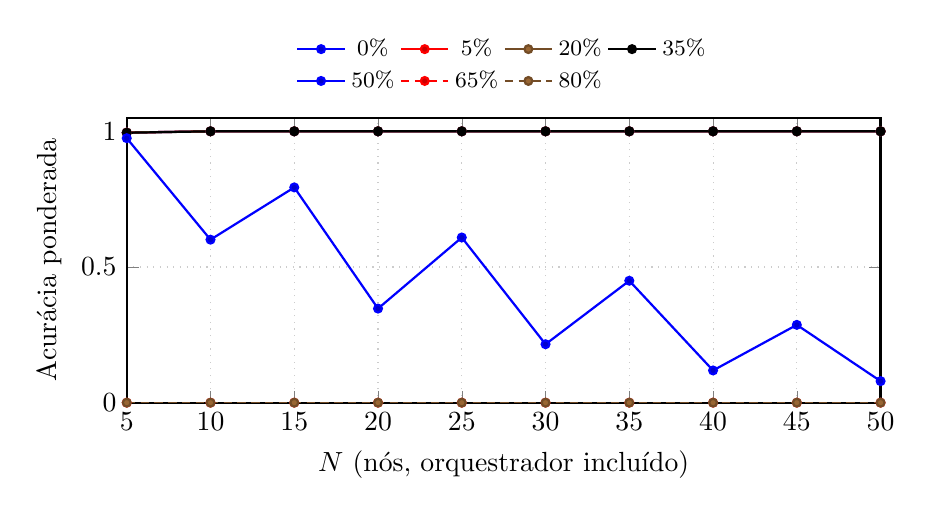
\begin{tikzpicture}
\begin{axis}[
  width=0.92\textwidth, height=5.2cm,
  ymin=0, ymax=1.05, xmin=5, xmax=50,
  xtick={5,10,15,20,25,30,35,40,45,50},
  xlabel={$N$ (nós, orquestrador incluído)},
  ylabel={Acurácia ponderada},
  grid=major, grid style={dotted,gray!40},
  legend style={font=\footnotesize, draw=none, fill=none, legend columns=4,
    at={(0.5,1.05)}, anchor=south},
  mark size=1.4pt, line width=0.8pt]
  \addplot+[mark=*] coordinates {(5,0.9953) (10,1.0000) (15,1.0000) (20,1.0000) (25,1.0000) (30,1.0000) (35,1.0000) (40,1.0000) (45,1.0000) (50,1.0000)};
  \addlegendentry{0\%}
  \addplot+[mark=*] coordinates {(5,0.9953) (10,1.0000) (15,1.0000) (20,1.0000) (25,1.0000) (30,1.0000) (35,1.0000) (40,1.0000) (45,1.0000) (50,1.0000)};
  \addlegendentry{5\%}
  \addplot+[mark=*] coordinates {(5,0.9953) (10,1.0000) (15,1.0000) (20,1.0000) (25,1.0000) (30,1.0000) (35,1.0000) (40,1.0000) (45,1.0000) (50,1.0000)};
  \addlegendentry{20\%}
  \addplot+[mark=*] coordinates {(5,0.9947) (10,1.0000) (15,1.0000) (20,1.0000) (25,1.0000) (30,1.0000) (35,1.0000) (40,1.0000) (45,1.0000) (50,1.0000)};
  \addlegendentry{35\%}
  \addplot+[mark=*] coordinates {(5,0.9747) (10,0.6007) (15,0.7933) (20,0.3467) (25,0.6087) (30,0.2153) (35,0.4493) (40,0.1187) (45,0.2867) (50,0.0793)};
  \addlegendentry{50\%}
  \addplot+[mark=*] coordinates {(5,0.0000) (10,0.0000) (15,0.0000) (20,0.0000) (25,0.0000) (30,0.0000) (35,0.0000) (40,0.0000) (45,0.0000) (50,0.0000)};
  \addlegendentry{65\%}
  \addplot+[mark=*] coordinates {(5,0.0000) (10,0.0000) (15,0.0000) (20,0.0000) (25,0.0000) (30,0.0000) (35,0.0000) (40,0.0000) (45,0.0000) (50,0.0000)};
  \addlegendentry{80\%}
\end{axis}
\end{tikzpicture}
\caption{Acurácia ponderada versus $N$ na configuração com conluio (sem instáveis).}
\label{fig:acuracia-conluio}
\end{figure}
